% !Mode:: "TeX:UTF-8"
\chapter{非稳态层流的数值模拟}

\section{问题描述}

\subsection{控制方程} % homogenous fluid region, and porous region

\subsection{边界条件} % Including interface between the homogeneous fluid and porous medium regions

\section{数值方法}

\subsection{时间和空间的离散方法}

\subsection{求解器} % SIMPLE

\subsection{网格生成和网格独立性分析}

流动区域设定为边长60的正方形。为了获得圆柱内外的流动状态,流动区域被划分为三块,其中有两块位于圆柱内部,一块位于圆柱外部,见图~\ref{fig: grid}。网格尺寸见表~\ref{tab: grid}。雷诺数和达西数分别为100和0.0001。
\begin{figure}[]
	\centering
	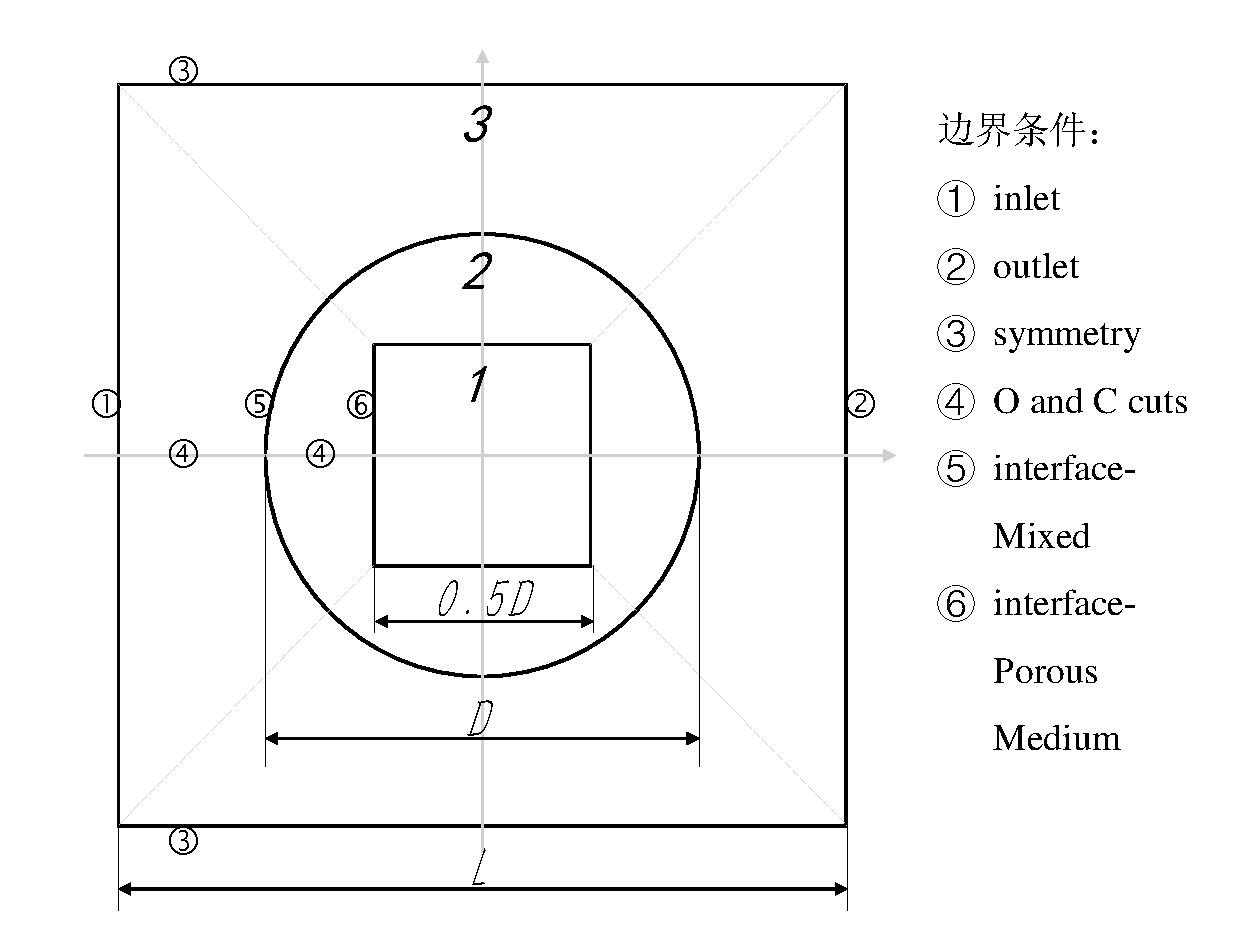
\includegraphics[scale=.6]{../diagrams/grid}
	\caption{网格划分}\label{fig: grid}
\end{figure}

\begin{table}[]
	\centering
	\caption{网格尺寸}\label{tab: grid}
	\begin{tabular}{@{}cccccc@{}}
		\toprule
		\multicolumn{2}{c}{Blocks}  & Block 1  & Block 2   & Block 3 & Mean drag coefficient    \\ \midrule
		\multirow{4}{*}{Grid size} 
		& Case 1 & 40 $\times$ 40 & 160 $\times$ 25 & 160 $\times$ 140   & 1.2354 \\
		& Case 2 & 60 $\times$ 60 & 240 $\times$ 30 & 240 $\times$ 170   & 1.2426 \\
		& Case 3 & 80 $\times$ 80 & 320 $\times$ 40 & 320 $\times$ 200   & 1.2462 \\
		& Case 4 & 100 $\times$ 100 & 400 $\times$ 50 & 400 $\times$ 230 & 1.2417 \\
		\bottomrule
	\end{tabular}
\end{table}

\section{本章小结}
